Now we discuss in details of our semantics interpretation of AGREE contracts with scheduled components.
\begin{figure}[ht!]
\centering
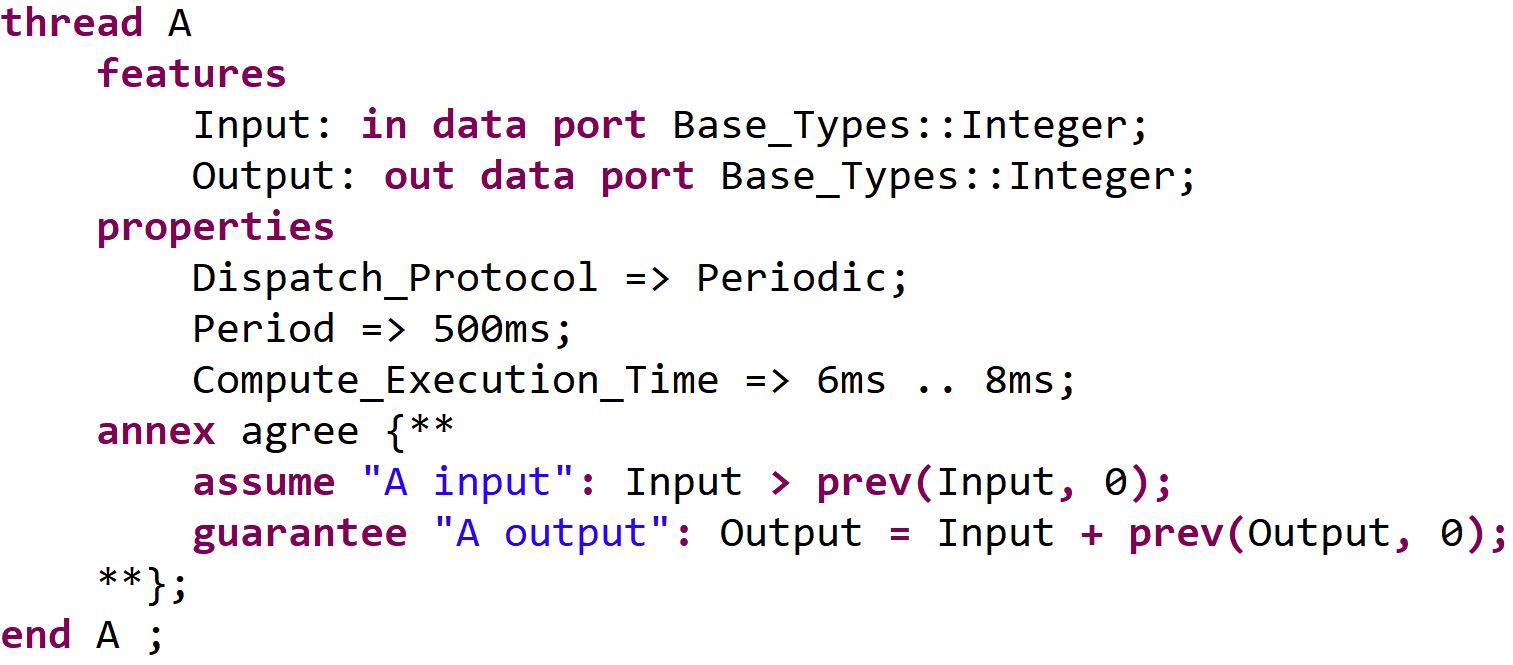
\includegraphics[width=80mm]{pre.jpg}
\caption{A Simple Integrator AADL Model in AGREE\label{integratorFig}}
\end{figure}

First, we use an example to illustrate our rationals. Consider the AADL model of an integrator shown in Figure \ref{integratorFig}. We assume an execution time slot in a schedule is assigned to the thread.  
The first question we have is when the contracts shall hold. In a synchronous model, contracts hold at every instant. However, with scheduled execution, it is reasonable to assume the contract may not hold when the component is not activated. But once it is activated, shall it hold throughout the whole execution or just at certain instants? Second, how shall $Input$ referred in the contract be interpreted? One interpretation is that it refers to the input value at the time when the contract is evaluated, which may vary during the execution. Another interpretation is that it refers to the input value when the component starts its execution. In other words, there is a notion of \emph{sample and hold}. Any input value change during the execution will not impact the current execution. This interpretation is consistent with the notion of \emph{frozen} input described in the AADL V2 standard. Third, how the \emph{prev} operator shall be interpreted? In a synchronous model, it refers to the previous instant. However, with scheduled execution, it seems reasonable to interpret \emph{prev} as previous activation (i.e. the last value when the component was activated). If the contracts hold throughout the activation, a more sensible interpretation is that at the first instant during activation, it refers to the previous activation. Then at each following instant, it refers to the last updated value in the current activation. This interpretation is adopted in the \emph{activation condition} in SCADE \cite{scade} or the \emph{clock} mechanism in SIGNAL \cite{signal}.

AGREE contracts are intended to model requirements \cite{AGREE2}, not implementations. Guarantees model the component requirements, and assumptions models the environmental constraints used to verify the component requirements. Following the AADL \emph{input-compute-output} model, we interpret that the assumptions shall hold at the start of the execution (i.e. \emph{dispatch}) when the inputs are read in. And the guarantees shall be satisfied at the end of the execution (i.e. \emph{complete}) when the outputs are written out. This interpretation has a few implications. 
First, since we adopt the AADL frozen input concept, any reference to $Input$ refers to the input value that was read in at dispatch.
Second, a component's assigned time slot does not necessarily match exactly with its execution time window. If the time slot is greater than its execution time, we interpret the start and end of the time slot as dispatch and complete, respectively. Otherwise, we interpret a preemption has occured.
Third, each contract is examined exactly once in each activation. Thus, we interpret the $prev$ operator as the previous activation. 
Examing guarantees only once means they are not intended to model the transient behavior during an execution. We interpret them as requirements on the steady-state outputs at the end of activation.

%This is different from the real-time behavior models used to formalize AADL semantics, like real-time Maude \cite{maude}, timed automata \cite{behaviorannex}, and timed Petri net \cite{tpn}. They model the component timing behavior throughout the whole execution. 
Note that this does not mean AGREE contracts cannot model timer (or integerator) based requirements. In practice, a timer is usually implemented as a counter, whose limit (constant) is calculated based on the frequency of its execution. The counter is activated periodically and increments by only one during each activation, independent of the execution time. This is consistent with our interpretation.

Thus, we introudce two distinctive events \emph{dispatch} and \emph{complete} for each component to model the start and end of its activation, respectively. 
Similarly, for a system (consists of components), the two events model the start and end of a scheduling cycle. 
The two events shall appear in pairs and alternately. dispatch shall appear before complete. We introduce \emph{well-orderedness} to capture the pattern.

In SCADE and SIGNAL, when a component is not activated, its outputs keep their previous values. We adopt the same notion of output freeze. The outputs are frozen between complete events. 

We inherit the communication mechnanism used in synchronous AGREE. The existence of a connection between two components means their contracts refer to the same variable. 
This essentially simulates an asynchronous communication between components with shared variable. It has one writer and possibly multiple readers. This is consisten with the AADL data port communication semantics.
Since the schedule ensures at most one component is activated at a time, there is no ambiguity on the order of read and write. For a preemptive schedule, we require a component can only be prempted by another component if they do not have connections.

The comminucation may also be viewed as a buffer of size one, which has exactly one writer and one reader. The writer overwrites when overflow occurs. The reader reads the last value if the queue is empty. This means the model only supports restrictive AADL event data port communication.

Following the AADL frozen input concept, we require the inputs values do not change while the component is activated. This implies assumptions could be examined at \emph{complete}, instead of \emph{dispatch}. Thus, we do not necessarily need introducing \emph{dispatch} event. We keep \emph{dispatch} event mainly for usability reasons. The (\emph{dispatch, complete}) pair helps users to understand a counterexample and mentally construct the system trace. This is particularly useful when the schedule is preemptive.

%{\bf Model of Real-Time Schedule.}
In practice, a schedule often orignally comes in form of a sequence of time slots associated wtih components. 
%The real-time schedule could come from an AADL scheduling tool like Cheddar \cite{Cheddar}, or from a scheduler provided by the RTOS/Microkernel verdor, like seL4\cite{seL4}. 
To properly model the schedule in AGREE, the component execution time has to be considered. Consider the example shown in Figure \ref{RTschedule}. There are two scheduled components $A$ and $B$. We refer the original schedule as real-time schedule. We refer its model in AGREE as AGREE schedule.
\begin{figure}[ht!]
\centering
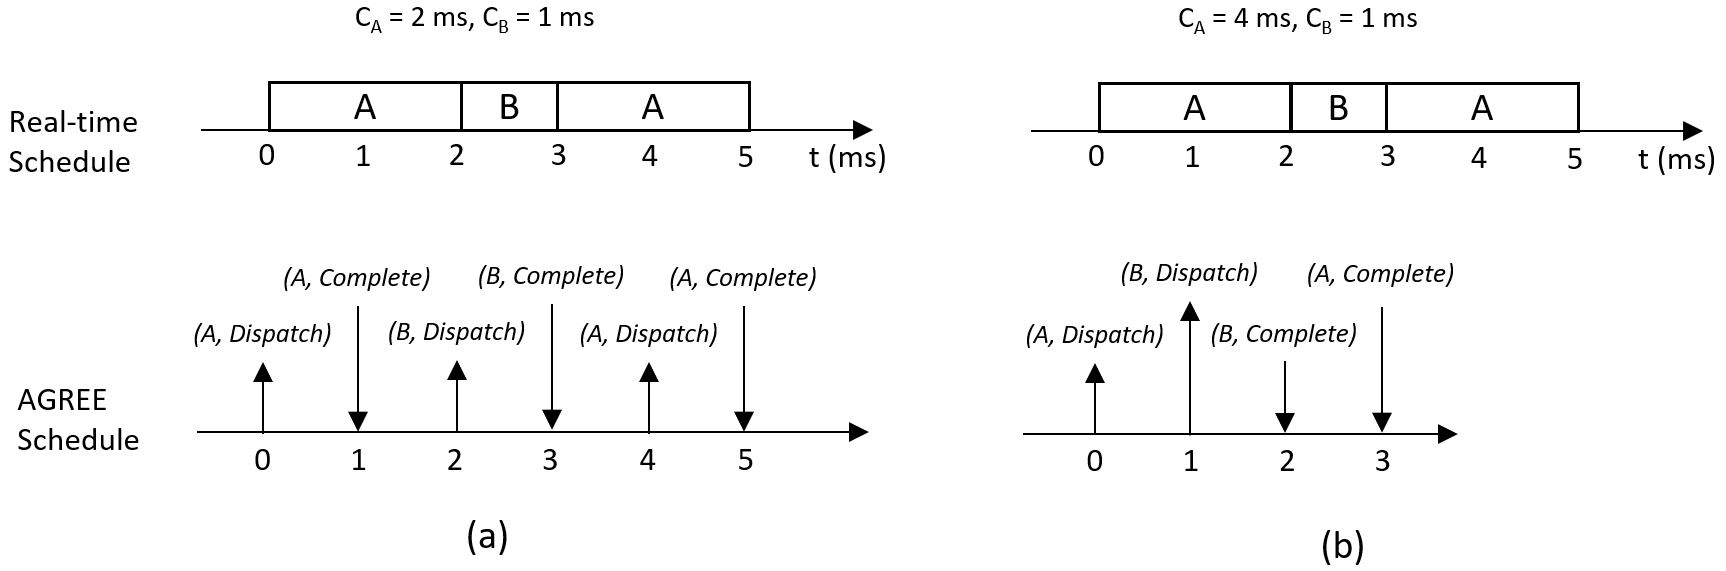
\includegraphics[width=130mm]{RTschedule.jpg}
\caption{A Model of Real-Time Schedule in AGREE\label{RTschedule}}
\end{figure}
Given the same real-time schedule, due to the different execution time $C_A$ of $A$, two different AGREE schedules are created. In Figure \ref{RTschedule}(a), since $C_A$ is equal to the time slots assigned to $A$, the end of the each time slot is modelled as \emph{complete}. In Figure \ref{RTschedule}(b), since the first time slot assigned for $A$ is less than its execution time, the end of the first time slot is interpreted as \emph{preemption}, instead of \emph{complete}.

%The AGREE reasoning framework uses past-time LTL [2], particularly LTL operator $G$ (globally), $H$ (historically), and $Z$ (previous). Given a component with an assume-gurantee pair ($A,P$) and an event pair (\emph{dispatch}, \emph{complete}), the meaning of the contract can be formally represented as a past-time LTL formula $G(H((dispatch \Rightarrow A)) \Rightarrow (complete \Rightarrow P))$. In synchronous AGREE, the two events \emph{collpase} into a single instant at each tick. Thus, we have $G(H(A) \Rightarrow P)$.

%A system consists of components, connections between components, contracts, and a schedule.
%The schedule defines a total order of dispatch and complete events of each component within a scheduling cycle.
%A valid schedule is one where component activations do not overlap.
%Once a component is activated, it runs to complete. There is no preemption.
%A component reads input at dispatch time. %Reading is non-blocking. It reads the most recent input data value or an initial value. 
%And the input is \emph{frozen} during the component activation.
%A component writes output at completion time. %Writing is non-blocking. It overwrites the previous data value. 
%And the output holds its data value between its completions.
%The connections represent an asynchrnous communication channel with a buffer of size one.
%The connections between components are unidirectional. %It represents communication through shared variable with one writer and possible multiple readers. 
%A component satisfies its assumptions at dispatch time. %If the assumption is violated, then the system is consided \emph{inconsistent}.
%A component satisfies its guarantees at completion time. 
%And the output holds its data value between its completions.


